% Appendix A

\chapter{Esquemáticos} % Main appendix title
\label{AppendixB} % For referencing this appendix elsewhere, use \ref{AppendixA}

\begin{sidewaysfigure}[!ht]
	\centering
	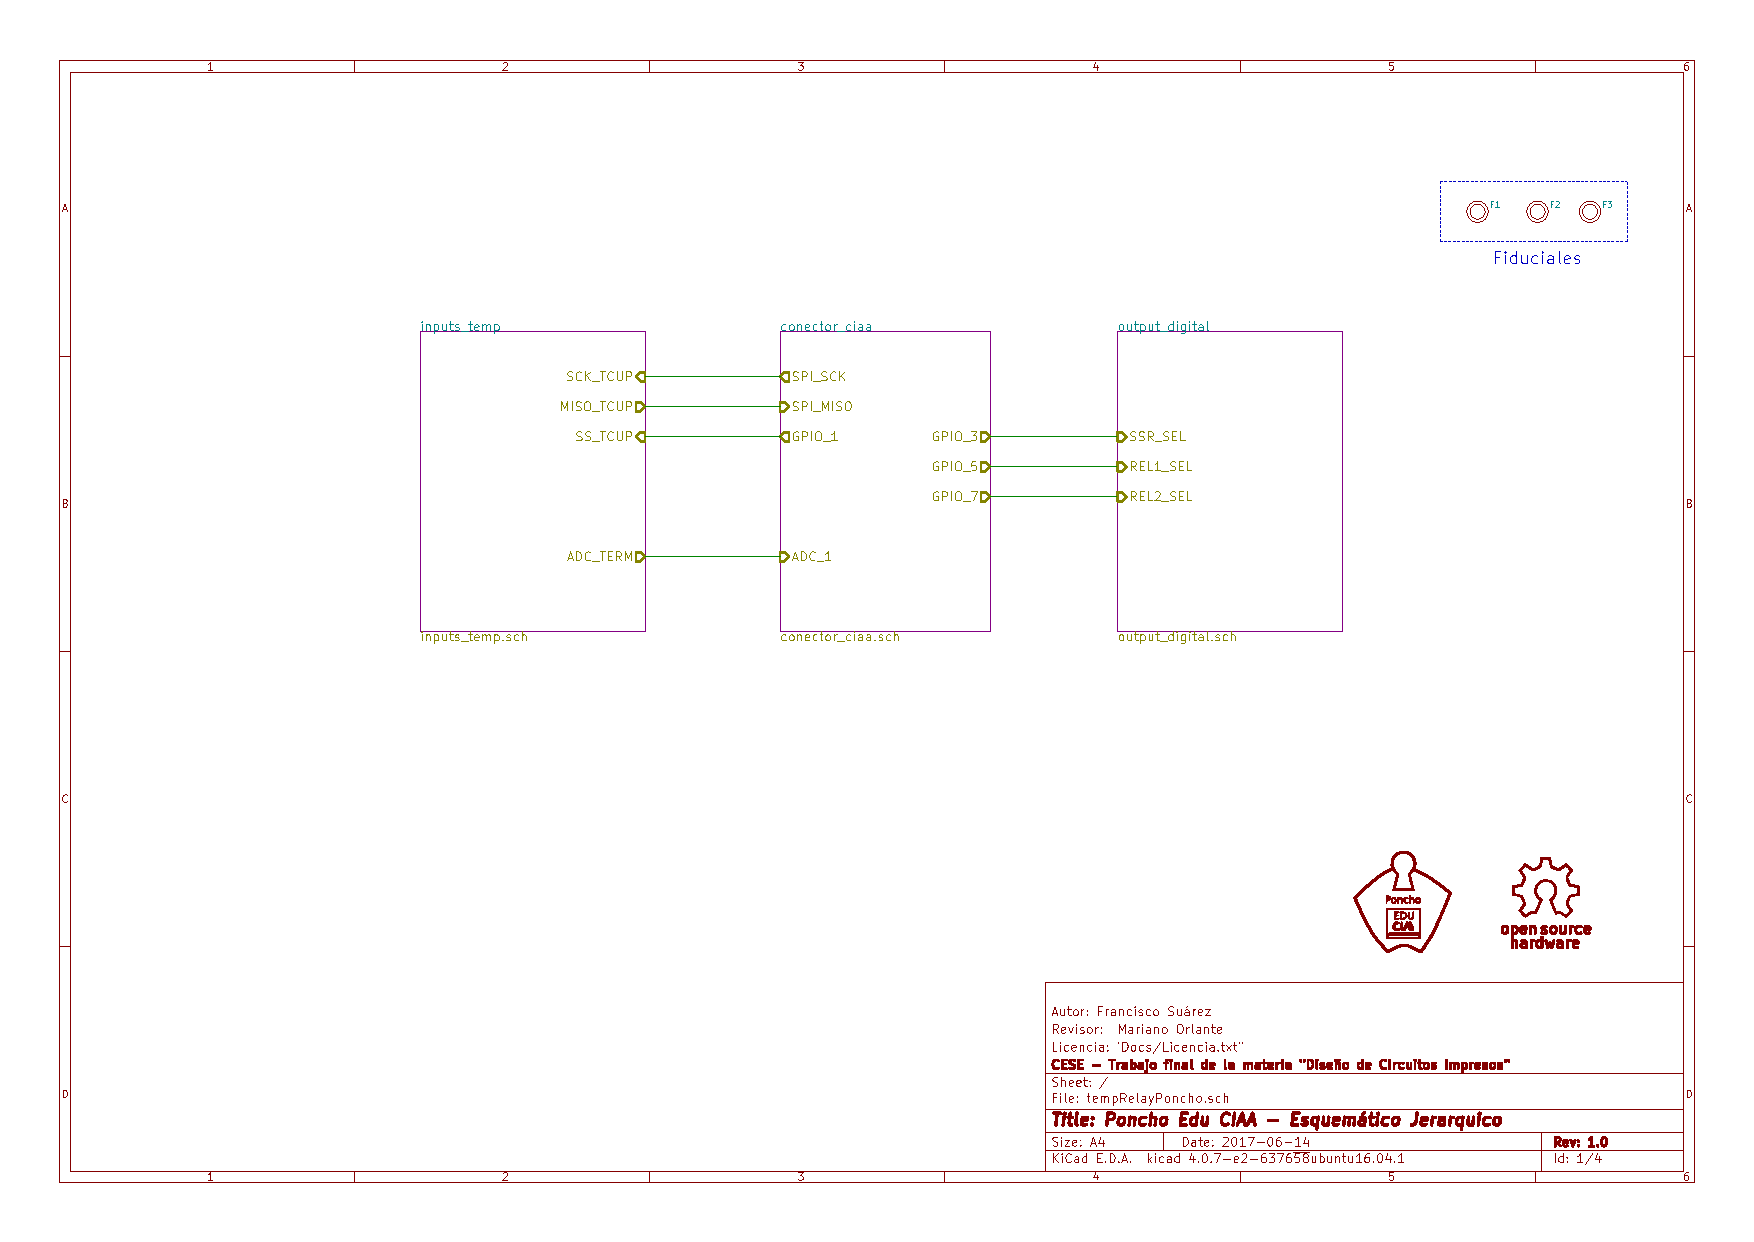
\includegraphics[width=0.9\textwidth]{Figures/Appendices/sch_mainPoncho}
	\caption{Esquemático jerárquico del poncho EduCiaa.}
	\label{fig:schMainPoncho}
\end{sidewaysfigure}


\begin{sidewaysfigure}[h!]
	\centering
	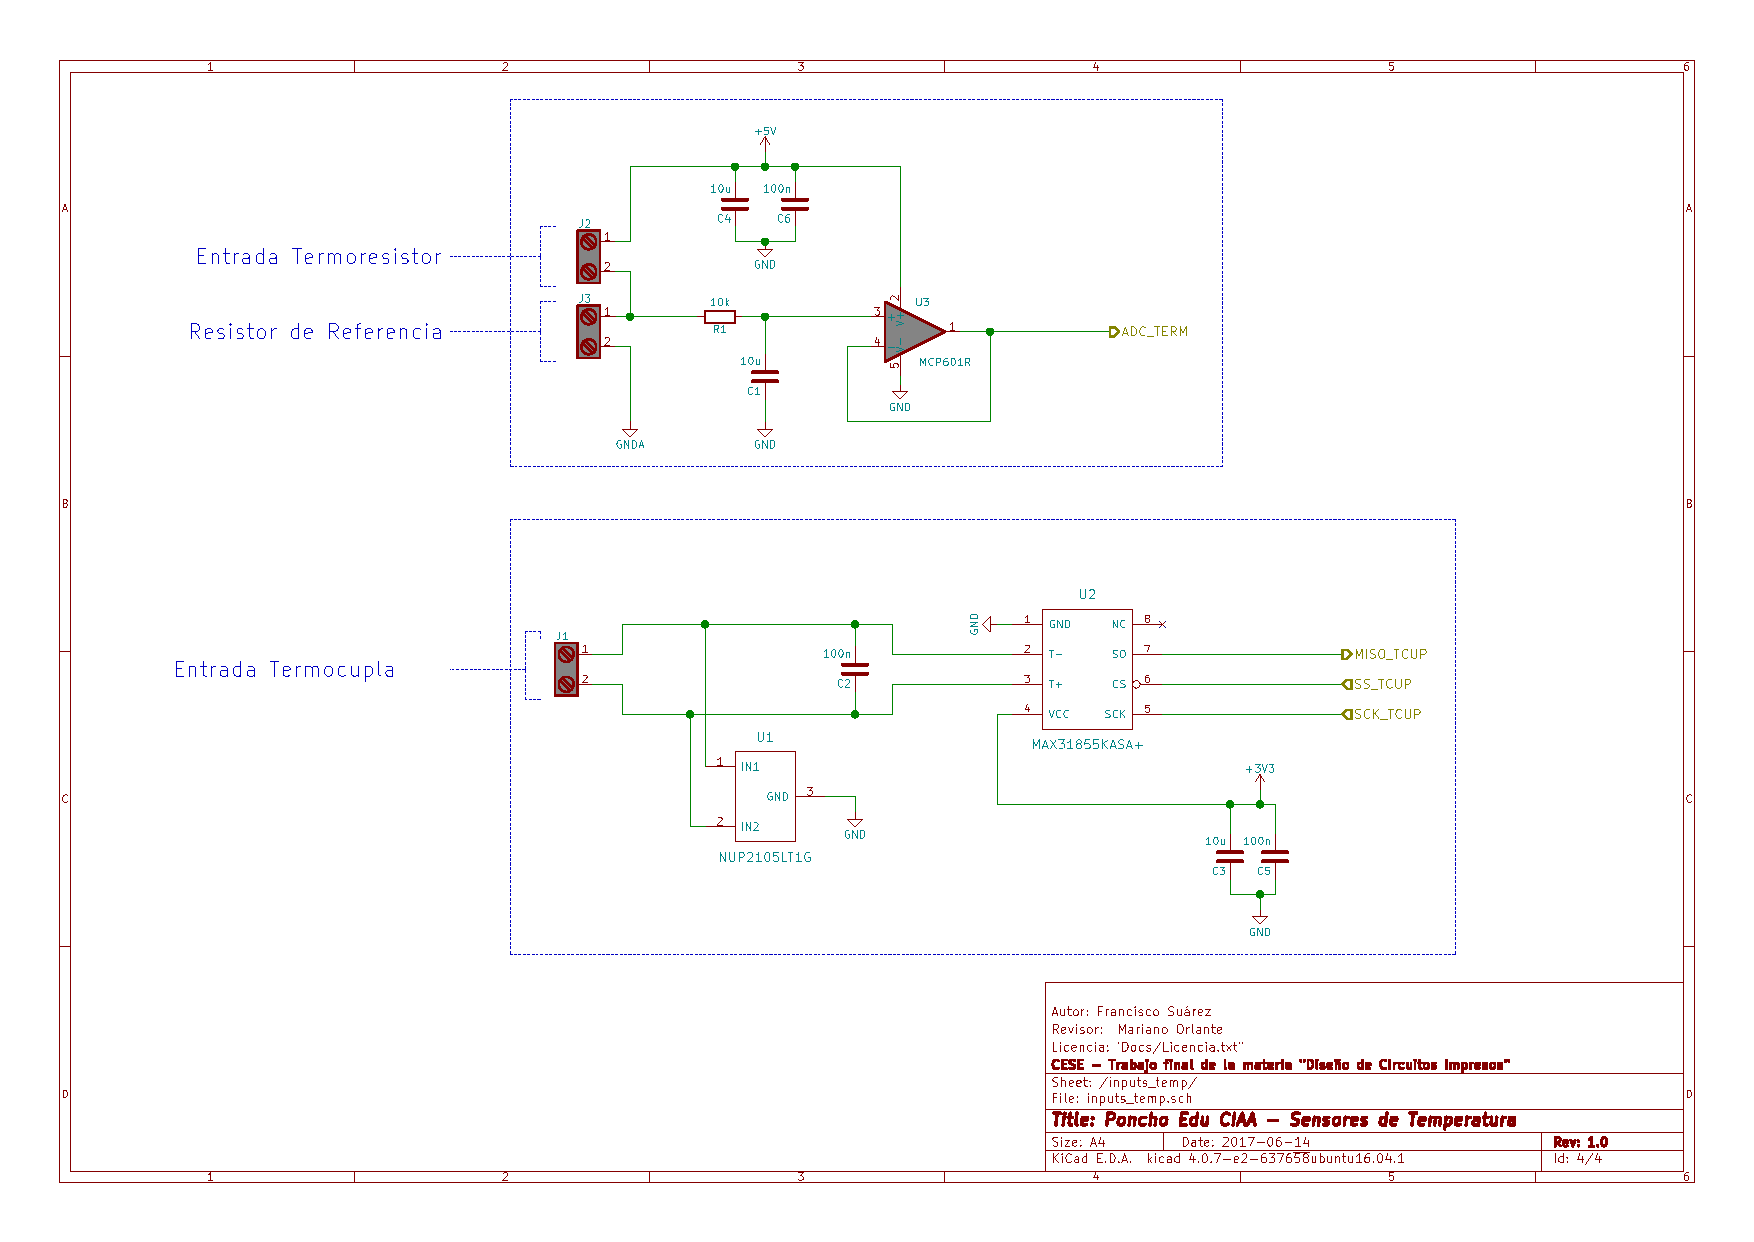
\includegraphics[width=1\textwidth]{Figures/Appendices/sch_inpTempTerm}
	\caption{Esquemático entradas de termocupla y termistor.}
	\label{fig:schEntradas}
\end{sidewaysfigure}


\begin{sidewaysfigure}[h!]
	\centering
	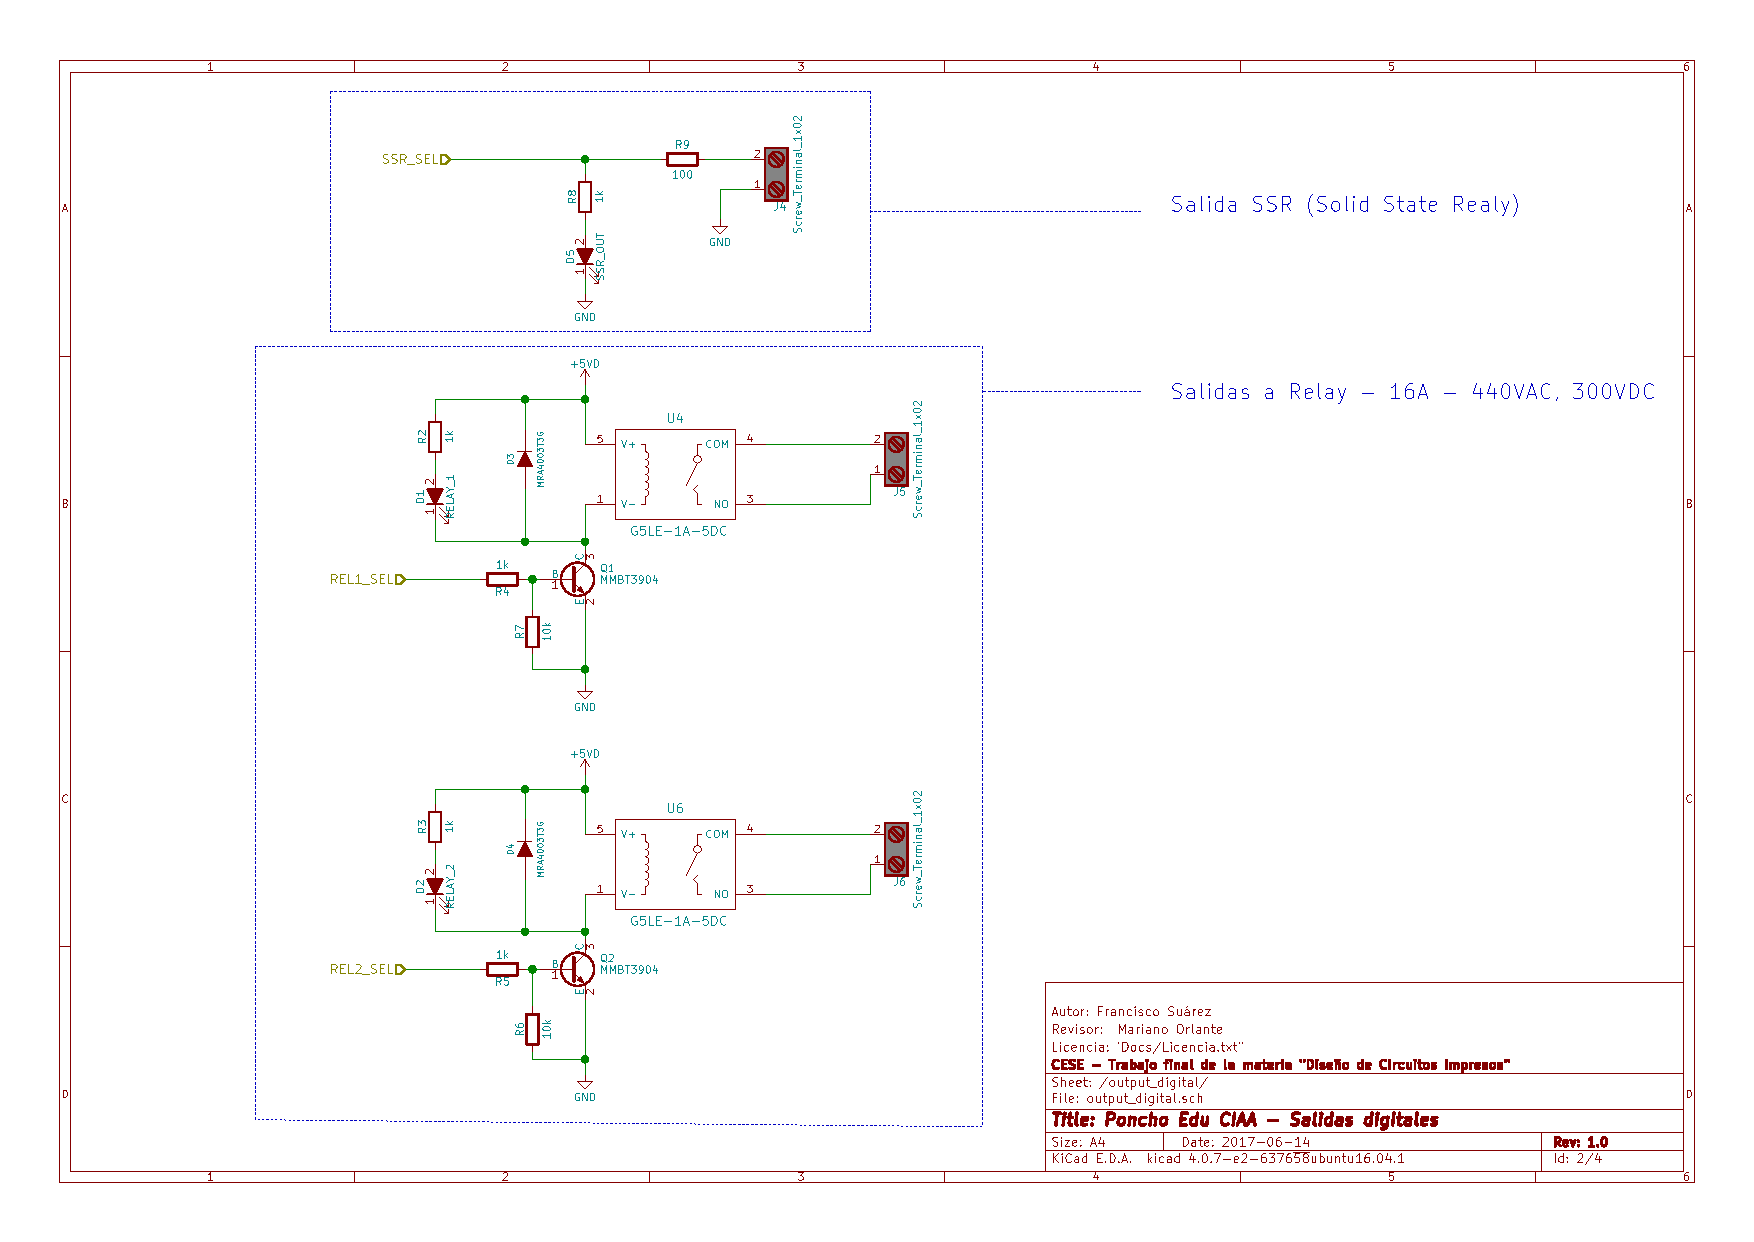
\includegraphics[width=1\textwidth]{Figures/Appendices/sch_outAnalogDigital}
	\caption{Esquemático de salidas digitales con relays.}
	\label{fig:schSalidas}
\end{sidewaysfigure}

\begin{sidewaysfigure}[h!]
	\centering
	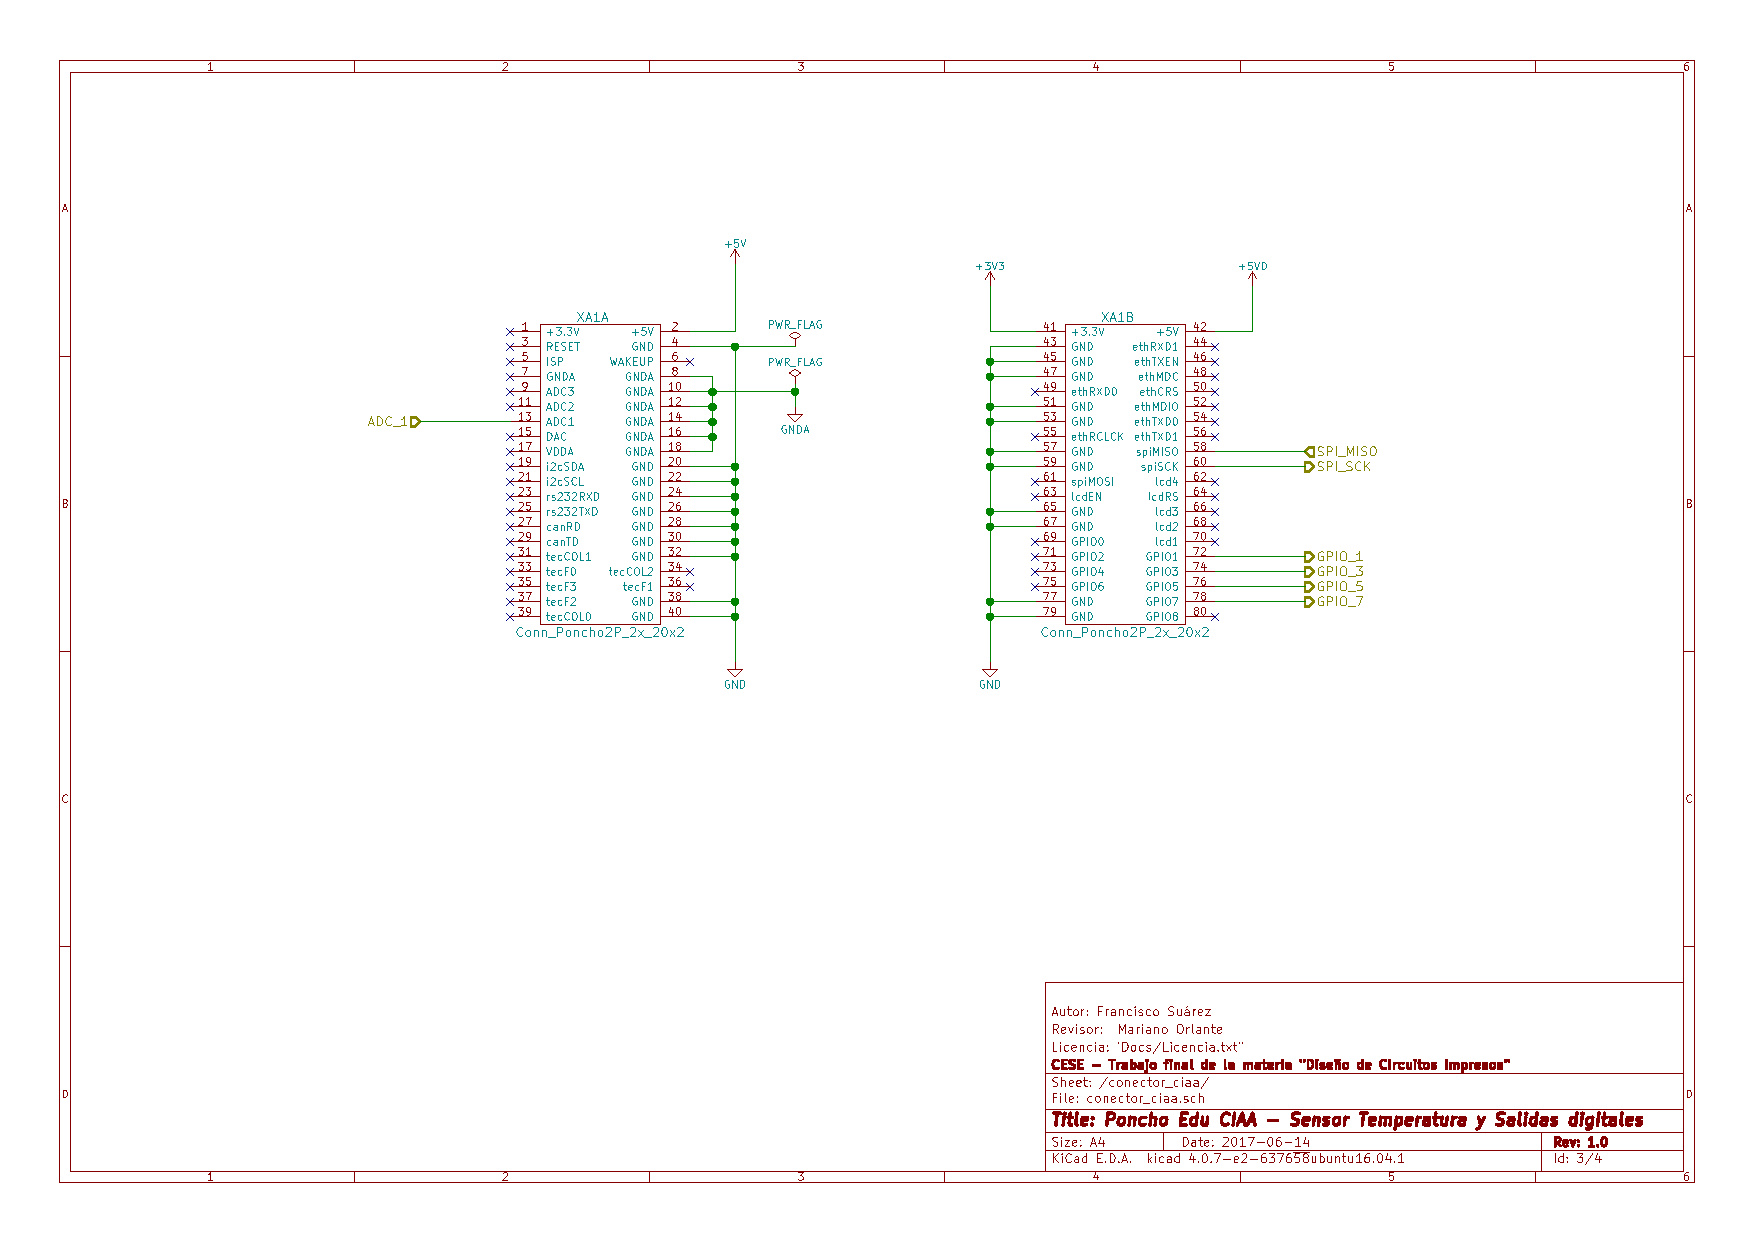
\includegraphics[width=1\textwidth]{Figures/Appendices/sch_conect_ciaa}
	\caption{Esquemático de conectores de expansión con la eduCIAA.}
	\label{fig:schSalidas}
\end{sidewaysfigure}


